\documentclass[uplatex, dvipdfmx]{jsarticle}
\usepackage{tikz}

\usetikzlibrary{arrows}
\usetikzlibrary{shapes.geometric}
\usetikzlibrary{positioning}
\usetikzlibrary{intersections, calc, arrows}

\begin{document}
\begin{figure}[h]
  \centering
  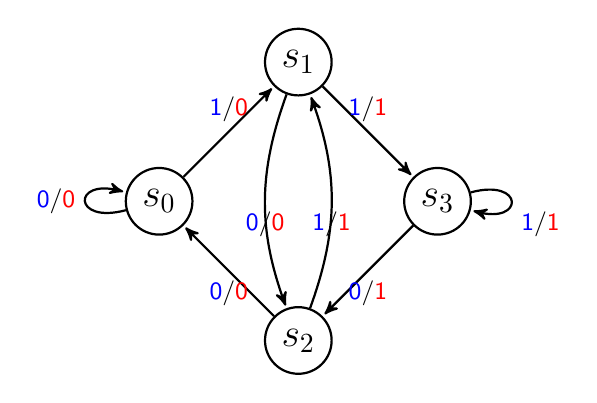
\begin{tikzpicture}[->,>=stealth',shorten >=1pt,auto,node distance=2.5cm,thick,
    square/.style={regular polygon,regular polygon sides=4},
    triangle/.style={regular polygon,regular polygon sides=3},
    pat node/.style={circle,draw,font=\sffamily\Large\bfseries},
    hos node/.style={triangle,draw,font=\sffamily\Large\bfseries},
    ext node/.style={square,draw,font=\sffamily\Large\bfseries}
    ]

    \node[pat node](0){$s_0$};
    \node[pat node](1)[above right of=0]{$s_1$};
    \node[pat node](2)[below right of=0]{$s_2$};
    \node[pat node](3)[below right of=1]{$s_3$};

    \path[every node/.style={font=\sffamily\small}]
    (0) edge[loop left] node[left]{\textcolor{blue}{0}/\textcolor{red}{0}} (0)
    (0) edge node[above]{\textcolor{blue}{1}/\textcolor{red}{0}} (1)
    (1) edge[bend right=20] node[below]{\textcolor{blue}{0}/\textcolor{red}{0}} (2)
    (1) edge node[above]{\textcolor{blue}{1}/\textcolor{red}{1}} (3)
    (2) edge node[below]{\textcolor{blue}{0}/\textcolor{red}{0}} (0)
    (2) edge[bend right=20] node[below]{\textcolor{blue}{1}/\textcolor{red}{1}} (1)
    (3) edge node[below]{\textcolor{blue}{0}/\textcolor{red}{1}} (2)
    (3) edge[loop right] node[below right]{\textcolor{blue}{1}/\textcolor{red}{1}} (3);
  \end{tikzpicture}
  \caption{状態遷移図}
  \label{graph}
\end{figure}
\end{document}
